%        File: learnability.tex
%     Created: Mon Feb 06 11:00 AM 2017 E
% Last Change: Mon Feb 06 11:00 AM 2017 E
%
% arara: pdflatex: {options: "-draftmode"}
% arara: biber
% arara: pdflatex: {options: "-draftmode"}
% arara: pdflatex: {options: "-file-line-error-style"}
\documentclass[MilwayThesis]{subfiles}

\begin{document}
In this section, I will evaluate some previous analyses of resultatives, based on their learnability, largely setting aside questions of over-/under-generation.
This choice of evaluation metric is motivated by the overall goals of this thesis and by the fact that questions of generative capacity are well-addressed by the analyses that I will evaluate.

The resultative parameter presents an acquisition problem for two broad reasons.
The first problem is that, on the surface, resultatives, which are parameterized, are indistinguishable from depictives, which appear to be universal.
The two construction types are indistinguishable in the sense that both correspond to the string template in \Next (modulo independent word order variation).
\ex. \textsc{Subj} V \textsc{Obj} Adj.

This indistinguishability is evident in the fact that one can construct examples which are truly ambiguous between resultative and depictive readings, as in \Next.
\ex. 
\a. He fried the fish dry.
\a. $\approx$ He fried the fish once it was dry. (\textbf{Depictive})
\b. $\approx$ He fried the fish until it was dry. (\textbf{Resultative})
\z.
\b. She painted the barn red.
\a. $\approx$ The barn is red in her painting. (\textbf{Depictive})
\b. $\approx$ She applied a coat of red paint to the door. (\textbf{Resultative})
\z.

Assuming a child acquiring either French or English encounters sentences with the form of \LLast in their PLD, there is no obvious way for the child to determine whether a given secondary predicate is to be interpreted depictively or resultatively.

An empiricist might object, arguing that the ambiguous examples above are highly constructed, and would easily by disambiguated in context.
They would insist that the learner would infer a positive setting of the resultative parameter from the use of a secondary predication construction in the presence of a resultative event.
So, an English learner, but not a French learner, might be exposed to the context-sentence pairing in \Next.
\ex. 
\a.[\textbf{Context:} ] A woman is methodically hammering a lump of metal.
A parent draws their child's attention to the hammering event and utters:
\b.[\textbf{A:}] She's hammering the metal flat.

Even this, however, is not fully unambiguous.
While it certainly couldn't be interpreted as a depictive, \textit{flat} could be interpreted as a manner adverb, modifying \textit{hammering}.
Such unavoidable ambiguity would make it difficult to employ any sort of semantic bootstrapping in the acquisition of the resultative parameter.

The second problem comes from the fact that both English-type and French-type languages can express resultative semantics periphrastically as in \Next.
\ex. (periphrasis)

The resultative parameter, then, is a one-or-both parameter, unlike other parameters which are either/or choices.
The verb raising parameter, for instance, is an either/or choice which can be made on the basis of the PLD:
If a learner encounters subject-verb inversion, they can infer that \textit{do}-support is impossible (at least for a given verb or verb class). 
If, however, a learner encounters \textit{do}-support, they can infer that subject-verb inversion is impossible. 
Turning to the resultative parameter, no such inference available to the learner:
The presence of a periphrastic resultatives in no way implies the impossiblity of adjectival resultatives, and vice versa.

One approach to the resultative parameter is what I will call the lexicalization account.
Under this account, event descriptions are decomposable into several universal features (\textit{e.g.}, \textsc{Result}, \textsc{Manner}, \textsc{Process}), and language variation results from languages lexicalizing these features differently.
One such an account by \textcite{son2008microparameters} proposes that English and German lexicalize \textsc{Result} in null heads, while Romance languages only lexicalize \textsc{Result} in verbs.
\ex.
\raisebox{-.9\height}{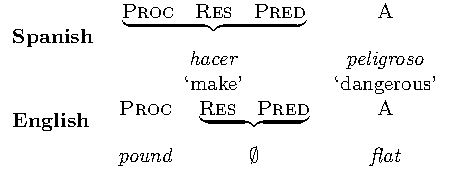
\includegraphics{lexicalization_table}}

Since the null LI is restricted to resultatives, the task of acquiring it depends on the learner distinguishing resultatives from depictives, and, as discussed above, such a task is far from trivial.

Indirect acquisition accounts of the resultative parameter, on the other hand, do not (necessarily) suffer from the drawbacks of direct acquisition.
The two that I will discuss -- \textcite{snyder2012parameter} and \textcite{kratzer2004building} -- both take Snyder's (\citeyear{snyder1995language}) compounding parameter as a starting point, but propose different sources of parameterization.
\textcite{snyder2012parameter} proposes that the parameter is the result of the (un)availability of a certain rule of semantic composition, while \textcite{kratzer2004building} argues that lexical variation is the cause of the resultative parameter.

\textcite{snyder2012parameter} proposes that the basis for The Compounding Parameter (TCP) is the (un)availability of a new rule of semantic composition: Generalized Modification, as defined in \Next.

\ex. Generalized Modification (GM)\\
If $\alpha$ and $\beta$ are syntactic sisters under the node $\gamma$, where $\alpha$ is the \uline{head} of $\gamma$, and if $\alpha$ denotes a \uline{kind}, then interpret $\gamma$ semantically as a \uline{subtype} of $\alpha$'s kind that stands in a pragmatically suitable \uline{relation} to the denotation of $\beta$
\quelle{\parencite[][underlining Snyder's]{snyder2012parameter}}

According to Snyder, GM is available in English-type languages and unavailable in French-type languages.
This amounts to two claims that I will address in turn below.
The first claim is that GM as defined in \Last is responsible for the phenomena that Snyder argues are covered by TCP (compounding, resultatives, particle verbs, etc.).
The second claim is that the availability of a given compositional rule varies parametrically.
Note that these claims are not of the same sort or import.
The first claim is a particular technical hypothesis, meaning it is open to adjustment should it prove imprecise or inaccurate.
If \Last is not the correct charecterization of TCP, it may be the case that something like \Last is.
The second claim is more broadly theoretical, meaning it is not adjustable.
So, if there is no variation in the availability of compositional rules, then the reality of GM is not obviously relevant to the characterization of TCP or the resultative parameter.

Snyder's claim that the CI interface is parameterized is an updated version of a claim he argues for in his \citeyear{snyder1995language} dissertation.
His claim is that, \textit{contra} the Borer-Chomsky conjecture, the cluster of variation he places under the umbrella of TCP cannot be reduced to lexical variation.
This claim, however, is based on a misinterpretation of the Borer-Chomsky Conjecture.
After describing the set of properties and arguing that they covary, Snyder asserts that ``[i]t is difficult to imagine that any single, independently motivated functional head will find a natural role both in complex predicates and in a morphological compound such as \textit{coffee cup}'' \parencite[62]{snyder1995language}.
I am inclined to agree with Snyder's assessment.
<++>

My argument against this has the following form:
(A) It is good scientific practice to admit only one explanation for a given phenomenon.
(B) There is strong evidence for the existence of lexical variation.
(C) The phenomenon that \textcite{snyder1995language} identifies can be given an explanation consistent with the Borer-Chomsky Conjecture.
If (B) and (C) are correct, (A) requires that we reject the claim that the CI interface is a locus of variation.

The bulk of this thesis is devoted to arguing for (C), and (A) is a methodological axiom, so I will restrict my comments in this section to (B).
The strength of the evidence of lexical variation is so great that it is often presupposed in any discussion of linguistic variation.
The difference between Mandarin and Cantonese is not \textit{merely} their lexicons.
Canadian English isn't \textit{just} British English with different words for things.
While it is true that the type of lexical variation we often presuppose is in the ``lexical'' inventory rather than the ``functional'' inventory that the Borer-Chomsky conjecture identifies as the locus of variation, there is also strong evidence that such variation exists.

Even if we restrict ourselves to English we can find many instances of functional variation.
Looking diachronically, we can see that the development of modern English from Old English involved a loss of case, gender and rich agreement morphology.
Syncronically, various dialects distinguish between second-person singular and plural pronouns, while Standard English does not.


%This account faces three problems:
%First, it does not properly capture the phenomenon of compounding.
%Second, parameterizing the syntax-semantics interface makes the acquisition task more difficult.
%Third, GM, as defined by Snyder, is not formulable as a principle of composition.
%I will discuss each of these issues below.
%
%According to Snyder's proposal, at least two things must be true of English: bare stems must be kind-denoting, and bare stem compounds must be kind denoting.
%Both requirements, however, are problematic.
%The first requirement -- that bare stems are kind-denoting -- at best, lacks independent evidence of its truth, and at worst, has significant evidence against its truth.
%If bare stems were kind-denoting, then we would expect to be able to use them to refer to kinds in English.
%Instead we see in \Next and \NNext that on mass noun bare-stems can be used to refer to kinds, while count nouns must be plural or embedded in singular definite DPs to be used to refer to kinds.
%\ex.
%\a. Water is essential.
%\b.* Dog is common.
%\c.* Dodo is extinct.
%
%\ex.
%\a.* Waters are essential.
%\b. Dogs are common.
%\c. The dodo is extinct.\\
%\quelle{\parencite[cf][]{chierchia1998reference}}
%
%Since bare stems are not generally kind-denoting in sentences, there is no reason to think they would be so in compounds.
%
%The second requirement of Snyder's proposal, that bare-stem compounds are kind-denoting, seems not to hold of English.
%Even if the prototypical compounds were kind-denoting (\textit{e.g.}, \textit{library book}), there is a class of compounds which are individual-denoting.
%These individual-denoting compounds are those which are headed by proper names like those in \Next.
%\ex.
%\a. Relationship George
%\b. <+More+>



\end{document}
